%===============================
%------------------------------
\section{Quantum Information and Ebits (Entanglement Bits)}
%------------------------------
%===============================

%---------------------------------------------
\subsection{Tensor product}
%---------------------------------------------

The quantum state of a joint system $AB$ lives in the tensor product space $\hilb_A\otimes \hilb_B$. The tensor product space can be defined without relying on specific bases on $\hilb_A$ and $\hilb_B$, but for the sake of simplicity, we will define the tensor product  via ONBs.

Suppose that $\{\ket{e_j}\}_j$ and $\{\ket{f_k}\}_k$ are ONBs for $\hilb_A$ and $\hilb_B$ respectively. (Their dimensions may not be the same.) $\hilb_A\otimes \hilb_B$ is simply the span (formal linear combinations) of elements in the Cartesian product $\{\ket{e_j}\}_j \times \{\ket{f_k}\}_k$, denoting the elements by $\ket{e_j}\otimes \ket{f_k}$.

A vector in $\hilb_A\otimes\hilb_B$ is said to be a {\bf product state} if it can be written as a simple product $\ket{\psi}\otimes\ket{\phi}$ of some $\ket{\psi}\in\hilb_A$ and $\ket{\phi}\in\hilb_B$. Otherwise, a vector is said to represent an {\bf entangled state}.
If needed, subscripts may be added to indicate which vector belongs to which Hilbert space, for example, $\ket{\psi}_A \otimes \ket{\phi}_B$. 
It is common to omit the tensor product symbol $\otimes$ and write a product state simply as $\ket{\psi}\ket{\phi}$, or even $\ket{\psi\phi}$ when no confusion may arise. The latter is extremely common when the qubit basis states are labeled by binary numbers, for example $\ket{00} = \ket{0}\otimes\ket{1}, \ket{01}=\ket{0}\otimes\ket{1}$, and so on.)
 
\vspace{0.5em}
\noindent {\bf Scalar multiplication}
\begin{align}
	\lambda(\ket{\psi}\otimes\ket{\phi}) &= 
	(\lambda\ket{\psi})\otimes\ket{\phi} =
	\lambda(\ket{\psi}\otimes(\lambda\ket{\phi}) 
\end{align}
\vspace{0.5em}
\noindent {\bf Vector addition}
\begin{align}
	(\ket{\psi_1} + \ket{\psi_2}) \otimes \ket{\phi} &= \ket{\psi_1} \otimes \ket{\phi} +  \ket{\psi_2} \otimes \ket{\phi} \\
\ket{\psi}\otimes(\ket{\phi_1} + \ket{\phi_2}) &= \ket{\psi}\otimes \ket{\phi_1}  + \ket{\psi}\otimes  \ket{\phi_2}	
\end{align}
Compare these to the rules \ref{direct-sum-add} and \ref{direct-sum-scalar} for the direct product (which is equivalent to the direct sum) of vector spaces.

Linear combinations of product vectors with no common factor (entangled states) are genuinely new objects in $\hilb_A \otimes \hilb_B$.

\vspace{0.5em}
\noindent {\bf Inner product.}
\begin{align}
	(\bra{\eta}\otimes\bra{\xi}) (\ket{\psi}\otimes\ket{\phi}) 
	= \av{\eta|\psi}\av{\xi|\phi}
\end{align}

\vspace{0.5em}
\noindent {\bf Partial inner product.}
\begin{align}
	{}_A\bra{\eta} (\ket{\psi}_A\otimes\ket{\phi}_B) 
	= \av{\eta|\psi}\ket{\phi}_B
\end{align}

\vspace{0.5em}
\noindent {\bf Linear operators.}
\begin{align}
	\op A\otimes \op B (\ket{\psi}\otimes\ket{\phi}) &= 
		(\op A\ket{\psi}) \otimes (\op B\ket{\phi}) \\
	(\op A \otimes \op B)(\op C\otimes \op D) &= (\op A \op C)\otimes (\op B \op D)
\end{align}
Thus, the trace factorizes.
\begin{align}
	\tr(\op A\otimes \op B) &= \sum_{jk} \bra{e_j} \bra{f_k} \op A\otimes \op B \ket{e_j}\ket{f_k} \\
	&= \sum_{jk} \mel{e_j}{\op A}{e_j} \mel{f_k}{\op B}{f_k} \\
	&= \tr(\op A) \otimes \tr(\op B)
\end{align}
\emph{Local operations} always commute.
\begin{align}
	[\op A\otimes \op\id, \op\id\otimes \op B] = \op A \otimes \op B - \op A \otimes \op B = 0
\end{align}
If one wants to represent a tensor product operator in a matrix form, one needs to fix the ordering of the bases of $\hilb_A \otimes \hilb_B$.\mn{By doing this, we are representing higher-rank tensors as a two-tensor (a matrix), and there is no canonical way to do it. It is more natural to represent them as they are, using quantum circuit diagrams or tensor diagrams \cite{coecke2009}.} When the lexicographic ordering is chosen, the matrix form has the form of the Kronecker product, which only shown here for the 2-by-2 case:
\begin{align}
	\op A \op B \longleftrightarrow \left(\begin{array}{c;{2pt/2pt}c}
		A_{00}B & A_{01}B \\ \hdashline[2pt/2pt]
		A_{10}B & A_{11}B 
	\end{array}\right).
\end{align}

\begin{mybox}
The concept of tensor product is typically introduced to students in a highly unintuitive setting of quantum theory, and as a result, the idea may appear alien at first. However, the tensor product is already present in ordinary probability theory as a self-evident means of combining the probabilities of two independent random variables.
\begin{align}
	\mqty(p \\ 1-p) \otimes \mqty(q\\1-q) = \mqty(pq \\ p(1-q) \\ (1-p)q \\ (1-p)(1-q))
\end{align}
In ordinary probability theory, a state that cannot be written as a product state $\ket{p}\otimes\ket{q}$ is a {\bf correlated state}. Entanglement is a form of correlation, but we will see in Section \ref{sec:A01} that it can be stronger than any classical correlation.
\end{mybox}

%---------------------------------------------
\subsection{Communication using entanglement}
%---------------------------------------------

The four {\bf Bell states} are defined to be
\begin{align}
	\ket{\Phi_{\pm}} &\equiv \frac{\ket{00}\pm\ket{11}}{\sqrt{2}}, \\
	\ket{\Psi_{\pm}} &\equiv 
	\frac{\ket{01}\pm\ket{10}}{\sqrt{2}}.
\end{align}
It is straightforward to verify that they form an ONB. Therefore, they constitute a basis measurement called the {\bf Bell measurement}.\mn{The Bell measurement is a prime example of a basis measurement that is not conventionally associated to any observable (i.e. a Hermitian operator).}
Alternatively, they can be arranged in a convenient form, 
\begin{align}\label{eq:steering}
	\ket{\Omega_{{\color{magenta}\tikzmark{a}a}{\color{eqcolor}\tikzmark{b}b}}} \equiv \op\id\otimes \op X^a\op Z^b \ket{\Omega},
\end{align}



\begin{tikzpicture}[remember picture,overlay]
	\draw[<-] 
	([shift={(2pt,-2pt)}]a) |- ([shift={(-10pt,-10pt)}]a) 
	node[anchor=east] {\scriptsize{\color{magenta}Parity bit}}; 
	\draw[<-] 
	([shift={(2pt,-2pt)}]b) |- ([shift={(14pt,-10pt)}]b) 
	node[anchor=west] {\scriptsize{\color{eqcolor}Phase bit}}; 
\end{tikzpicture}


\noindent obtained from  $\ket{\Omega}\equiv \ket{\Phi_+}$ via a local Pauli operation. In particular,
\begin{align}
	\ket{\Omega_{00}} &= \op\id\otimes\op\id\ket{\Omega} = \frac{\ket{00}+\ket{11}}{\sqrt{2}}, \\
	\ket{\Omega_{01}} &= \op\id\otimes\op Z\ket{\Omega}= \frac{\ket{00}-\ket{11}}{\sqrt{2}}, \\
	\ket{\Omega_{10}} &= \op\id\otimes\op X\ket{\Omega}= \frac{\ket{01}+\ket{10}}{\sqrt{2}}, \\
	\ket{\Omega_{11}} &= \op\id\otimes\op X \op Z\ket{\Omega}= \frac{\ket{01}-\ket{10}}{\sqrt{2}}.
\end{align}

\begin{lemma}\label{}
	For any linear operator $\op T$,
	\begin{align}
		\op\id\otimes \op T\ket{\Omega} = \op T^t \otimes \op\id \ket{\Omega},
	\end{align}
	where $^t$ denotes the matrix transposition in the standard basis $\{\ket{0},\ket{1}\}$. In particular, we have that
	\begin{align}
		\ket{\Omega_{11}} = \op\id\otimes \op X\op Z\ket{\Omega} = \op Z\op X \otimes \op\id \ket{\Omega}.
	\end{align}
\end{lemma}

\begin{proof}
    \begin{align}
       \op\id\otimes\op T\sum_j \ket{j}_A \ket{j}_B &= \sum_{jk} \ket{j}_A \ket{k}_B\bra{k} \op T \ket{j}_B \\
       &= \sum_k \underbrace{\sum_j  (T^t)_{jk} \ket{j}_A}_{\op T^t \ket{k}_A}\ket{k}_B
       = \op T^t \otimes \op\id \ket{\Omega}
    \end{align} 
\end{proof}


In the followings, we suppress the tensor product symbol when writing two-body Pauli operators: $\op \sigma_j \op \sigma_k = \op \sigma_j \otimes \op \sigma_k$.
Since
\begin{align}
	\op Z\op Z\ket{x_1}\ket{x_2}=(-1)^{x_1\oplus x_2}\ket{x_1}\ket{x_2}, && 
	\op X\op X\ket{x_1x_2}=(-1)^{x_1\oplus x_2}\ket{x_1\oplus 1}\ket{x_2\oplus 1},
\end{align}
we can see that $\op Z \op Z$ measures the parity bit and $\op X \op X$ measures the phase bit,
\begin{align}
	\op Z\op Z \ket{\Omega_{ab}} &= (-1)^a \ket{\Omega_{ab}}, \\
	\op X\op X \ket{\Omega_{ab}} &= (-1)^b \ket{\Omega_{ab}}.
\end{align}
For $\op Y \op Y$, note that
\begin{align}
	-\op Y \op Y =  (\op Z \op Z)(\op X \op X).
\end{align}
Therefore
\begin{align}
		-\op Y\op Y \ket{\Omega_{ab}} &= (-1)^{a\oplus b} \ket{\Omega_{ab}}.
\end{align}

Special attention should be paid to the {\bf singlet state} $\ket{\Psi_-} = (\ket{01}-\ket{10})/\sqrt{2}$ with the property that simultaneous spin measurements on the two qubits in the same direction are always \emph{anti-correlated}. In particular, the state can be written as
\begin{align}
	\frac{\ket{\hat{\vb n}}\ket{-\hat{\vb n}} - \ket{-\hat{\vb n}}\ket{\hat{\vb n}}}{\sqrt 2}
\end{align}
The singlet state can be prepared, for instance, via the process of spontaneous parametric down-conversion (SPDC) that produces a photon pair with opposite polarizations.



\begin{example}[\bf Superdense coding]\leavevmode
	
	Equation \eqref{eq:steering} implies that if Alice and Bob possess an entangled pair $\ket{\Omega}$, Alice can communicate two bits of information (the parity bit and the phase bit) to Bob by choosing to perform a Pauli operation on her side and send the qubit to Bob. In the form of \emph{Bennett's law}, we state that
	\begin{align}\label{eq:superdense}
		\textrm{1 ebit + 1 qubit} \succ \textrm{2 bits},
	\end{align} 
	where $\succ$ means ``can perform a task in place of".
\end{example}

\begin{example}[\bf Teleportation]\leavevmode
	
	The ``converse" to \eqref{eq:superdense},
		\begin{align}\label{eq:teleport}
		\textrm{1 ebit + 2 bits} \succ \textrm{1 qubit},
	\end{align} 
	is \emph{quantum teleportation}. Alice and Bob again begins the protocol with a pre-shared entanglement $\ket{\Omega}$, but now Alice has an unknown state $\ket{\psi}$ that she wants to send to Bob. Rather than sending the qubit directly (which would need a high-fidelity quantum channel, for example), what Alice can do is performing the Bell measurement on her unknown state and one half of the Bell pair. Remarkably, depending on the two-bit outcome $ab$ that Alice obtained, the post-measurement state on Bob's side becomes
	\begin{align}
		\ket{\psi'} = \op X^b \op Z^a \ket{\psi},
	\end{align}
which is not exactly the state $\ket{\psi}$ that Alice wants to send, but the extra Pauli operators can be corrected away with the information of the bits $ab$ that Alice can tell Bob by calling him on a phone, for example.
\end{example}
	
Proofs of the teleportation protocol found in textbooks are often quite long and involve some unintuitive steps. The following short proof is inspired from the tensor diagrammatic proof \cite{coecke2009}.
Let the subscripts $A,B$, and $C$ denote the Hilbert space of Alice's unknown qubit state, the Hilbert space of one half of the Bell pair that Alice holds, and the Hilbert space of the other half of the Bell pair that Bob holds, respectively.  
	\begin{align}
		{}_{AB}\bra{\Omega_{ab}} \left(\ket{\psi}_A \ket{\Omega_{00}}_{BC}\right)
		&= \frac{1}{2} \left[\sum_j \bra{j}_A \bra{j}_B(\op Z^a \op X^b)_A\dgg \otimes \op \id_B\right] \ket{\psi}_A \sum_k \ket{k}_B \ket{k}_C \\
		&= \frac{1}{2} \sum_{jk} \bra{j}_A\underbrace{\op X^b \op Z^a \ket{\psi}_A}_{\ket{\psi'}} \underbrace{\bra{j}_B\ket{k}_B}_{\delta_{jk}} \ket{k}_C\\
		&= \frac{1}{2} \sum_j \braket{j}{\psi'} \ket{j}_C\\
		&= \frac{1}{2} \ket{\psi'}_C
	\end{align}
	The subnormalization factor 1/2 tells us that the outcome probabilities for the Bell measurement are uniform.


%---------------------------------------------
\subsection{EPR argument}
%---------------------------------------------

A philosophical troubling aspect of quantum theory is that one cannot in general think of an act of measuring as revealing a pre-existing value of the measured property. When the system is in an eigenstate of an observable $\hat A$ with an eigenvalue $\lambda$, subsequent measurements of $\hat A$
do not alter the state, hence there is a tendency to think of the value $\lambda$ as pre-existed. Einstein, Padolsky, and Rosen (EPR) devised a clever argument using quantum correlation and the principle of relativity to argue that values of incompatible (non-commuting) observables can simultaneously pre-exist.
\begin{figure}[h]
	\centering
	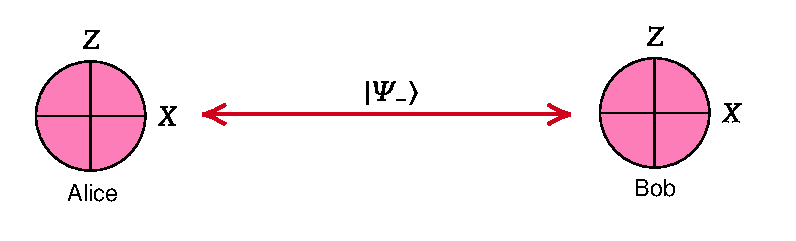
\includegraphics[scale=0.75]{fig/epr-measurement-setting}
	\caption{Measurement settings in the EPR argument.}
	\label{fig:epr-setting}
\end{figure}

The singlet state $\ket{\Omega_{11}}$ is an eigenstate shared by $\op Z\op Z$ and $\op X\op X$ with both eigenvalues -1. (Verify that they commute.) Now, while Alice cannot make a local Z and X measurements at the same time, if she chooses to measure one, say $\op Z_A$ and find the value $z_A = \pm 1$, then the spin of Bob's particle would need to have the opposite value to satisfy $z_A z_B =-1$. Since the spins are anti-correlated in every direction in the singlet stat, the same conclusion follows if Alice were to measure $\op X_A$. But, EPR argued, the act of measurement by Alice over here cannot effect the state of Bob's particle over there. Thus, the fact that Alice could have chosen to measure either observable and inferred $z_B$ or $x_B$ without disturbing Bob's particle means that those values already existed before the measurement.

\begin{align*}
	\left(\parbox{8em}{\centering {\bf Entanglement} \\ Anti-correlation \\ in the singlet state}\right)
	+ \left(\parbox{8em}{\centering {\bf Relativity} \\ The choice of measurement on A cannot have an influence on B}\right)
	\implies 
	\left(\parbox{8em}{\centering {\bf Quantum theory is incomplete}}\right)
\end{align*}

\noindent The EPR correlation in the $Z$ and $X$ measurement outcomes can be explained by classical hidden variables, in particular, Spekkens' toy theory \cite{spekkens2007}. See also \cite{wood2015} for diagrams similar to Figures \ref{fig:epr-setting} and \ref{fig:chsh-setting}.

%---------------------------------------------
\subsection{CHSH inequality}\label{sec:chsh}
%---------------------------------------------

The hope that quantum theory can be completed with \emph{hidden variables} that behave entirely classically is dashed by an experimental violation of the CHSH inequality.\mn{Named after John Clauser, Michael Horne, Abner Shimony, and Richard Hol, the inequality is formulated to be more suitable for experimental tests, an improvement over Bell's inequality.} Here we present a derivation of the CHSH inequality in the setting of a communication game, called a \emph{nonlocal game} in this context \cite{bell-nonlocality-review}.

Consider a communication game involving two players, Alice and Bob. In this cooperative game, Alice and Bob initially have the opportunity to consult and share their strategies before separating and traveling to two distant referees. The players are allowed to communicate in advance, but once the game begins, they are unable to communicate due to the restriction imposed by the speed of light.

\vspace{0.5em}
\noindent {\bf Game structure.}
At the referee stations, two binary questions are randomly chosen, denoted by $x\in\{0,1\}$ for Alice's question and $y\in\{0,1\}$ for Bob's question. Alice and Bob must give answers immediately, represented by variables $a\in\{0,1\}$ and $b\in\{0,1\}$, respectively. Because of the random choices, neither player knows the question in advance, and they cannot communicate the questions they received fast enough to change their answers. The referees then record the answers and later compare notes.

\vspace{0.5em}
\noindent {\bf Winning Condition.}
The goal for Alice and Bob to win the game is for the logical AND of their answers $a\wedge b$ to be equal to the product  of the choices of the questions $xy$. Here, $a\wedge b$ represents whether the answers agree (0) or disagree (1). In other words, they win if the following condition is satisfied:
\begin{align}
	xy = a\wedge b.
\end{align}
The only instance where Alice and Bob's answers must disagree is when $x=y=1$, see Figure \ref{fig:chsh}. 
\begin{marginfigure}
	\centering
	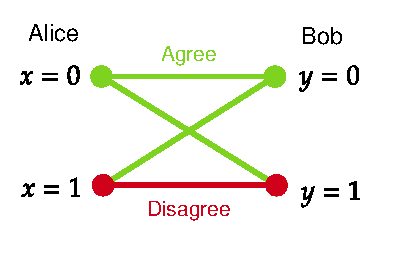
\includegraphics[scale=0.75]{fig/chsh.pdf}
	\caption{Diagram illustrating the rule of the nonlocal game.}
	\label{fig:chsh}
\end{marginfigure}
The agreement-disagreement relationship between the questions and answers forms a \emph{frustration graph}. It becomes evident that it is impossible to assign simultaneous edge values ($a$ and $b$) to satisfy the winning condition. In the case of a deterministic strategy where Alice and Bob always answer yes or no, the game can be won with a probability of 3/4. Remarkably, this represents the best achievable winning probability for Alice and Bob. (The winning probability for mixed strategies is at most equal to that of deterministic strategies.)
This bound on the winning probability
\begin{align}
	\Pr_{\substack{\textrm{win}\\ \textrm{classical}}} \le \frac{3}{4}.
\end{align}
is one form of the CHSH inequality; it signifies the limit of any classical local hidden variable theory.
\begin{align*}
	\left(\parbox{5.5em}{\centering {\bf Classical correlation} }\right)
	+ \left(\parbox{8em}{\centering {\bf Relativity} \\ The choice of measurement on A cannot have an influence on B}\right)
	\implies 
	\left(\parbox{8em}{\centering {\bf CHSH inequality}}\right)
\end{align*}

Now we show that if Alice and Bob have shared the singlet state beforehand, they can win the game with a probability greater than what is permissible by the CHSH bound.
\begin{figure}[h]
	\centering
	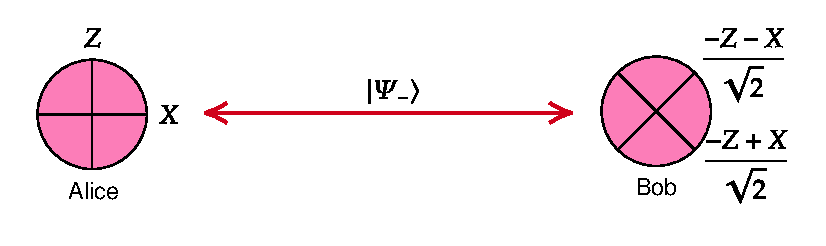
\includegraphics[scale=0.75]{fig/chsh-measurement-setting}
	\caption{Measurement settings that leads to a violation of the CHSH inequality given that Alice and Bob pre-shared the singlet state.}
	\label{fig:chsh-setting}
\end{figure}
\begin{align}
	\Pr_{\textrm{win}} &= \frac{1}{4}(p_{00}^{(+)} + p_{01}^{(+)} + p_{10}^{(+)} + p_{11}^{(-)}) \\
	&= \frac{1}{4}\av{\op P_{00}^{(+)} + \op P_{01}^{(+)} + \op P_{10}^{(+)} + \op P_{11}^{(-)}}
\end{align}
Solve for $\op P^{(\pm)}$ in terms of the observables.
\begin{align}
	\begin{cases}
		\op P^{(+)} + \op P^{(-)} &= \op \id, \\
		 \op P^{(+)} - \op P^{(-)} &= \op \sigma_{xy},
	\end{cases}
	\implies \op P^{(\pm)} = \frac{\op\id + \op\sigma_{xy}}{2}
\end{align}
Thus,
\begin{align}
	\Pr_{\textrm{win}} &= 
	\frac{1}{2} + \frac{1}{8}\av{\op\sigma_{00} + \op\sigma_{01} + \op\sigma_{10}  - \op\sigma_{11}}. 
\end{align}
Specialize to the measurement angles given in...
\begin{align}
\Pr_{\textrm{win}} &=   \frac{1}{2} + 
	\frac{1}{8}\av{\op Z\otimes \frac{-\op Z + \op X}{\sqrt 2} 
	+ \op Z\otimes \frac{-\op Z - \op X}{\sqrt 2}
	+ \op X\otimes \frac{-\op Z + \op X}{\sqrt 2}
	- \op X\otimes \frac{-\op Z - \op X}{\sqrt 2}} \\
	&=  \frac{1}{2} + 
	\frac{1}{8\sqrt 2} \av{\op Z\op Z + \op X \op X} = \frac{1}{2} + \frac{\sqrt 2}{4} \approx 85\% >
	\frac{3}{4} \ge \Pr_{\substack{\textrm{win}\\ \textrm{classical}}},
\end{align}
where the expectation value is taken with respect to the singlet state.

The original form of the CHSH inequality, $S_{\textrm{classical}} \le 2$, is phrased in terms of expectation values, especially two-point correlation functions,
\begin{align}
	S = \abs{\av{\op \sigma_{00}} + \av{\op \sigma_{01}} + \av{\op \sigma_{10}} - \av{\op \sigma_{11}}}.
\end{align}
The maximum violation allowed by quantum theory is $S = 2\sqrt{2}$, which is what we achieved in the computation above, called the \emph{Tsirelson bound}. The winning probability of 1 corresponds to the value $S=4$, which is achievable in non-quantum theories that, surprisingly enough, still do not violate special relativity (called \emph{non-signaling theories}) \cite{pr-box}. However, there can be some highly unlikely consequences in a universe in which such  \emph{super-quantum} theory is obeyed such as trivial communication complexity \cite{vandam2012}.


